\documentclass[aspectratio=169,12pt]{beamer}
\usetheme{Madrid}
\usecolortheme{whale}
\setbeamertemplate{navigation symbols}{}
\setbeamertemplate{footline}[frame number]

\usepackage[utf8]{inputenc}
\usepackage{amsmath,amsfonts,amssymb}
\usepackage{graphicx}
\usepackage{booktabs}
\usepackage{tikz}
\usepackage{array}
\usepackage{xcolor}

% colours
\definecolor{accent}{HTML}{1565C0}
\definecolor{good}{HTML}{2E7D32}
\definecolor{bad}{HTML}{C62828}
\setbeamercolor{title}{fg=white,bg=accent}
\setbeamercolor{frametitle}{fg=white,bg=accent}
\setbeamercolor{block title}{fg=white,bg=accent!80!black}
\setbeamercolor{block body}{bg=accent!5}

\newcommand{\highlight}[1]{\textcolor{accent}{\textbf{#1}}}
\newcommand{\good}[1]{\textcolor{good}{\textbf{#1}}}
\newcommand{\bad}[1]{\textcolor{bad}{\textbf{#1}}}

\title[Two-Phase PageRank]{\Large Two-Phase PageRank\\with Travel-Time Self-Loops}
\subtitle{Traffic Prediction on the Salt Lake City Road Network}
\author{Hamid}
\date{\today}

\begin{document}

%=================================================================
\begin{frame}
  \titlepage
\end{frame}

%=================================================================
\begin{frame}{Outline}
  \tableofcontents
\end{frame}

%=================================================================
\section{Problem \& Approach}
%=================================================================

\begin{frame}{The Traffic Prediction Problem}
  \begin{columns}[T]
    \begin{column}{0.55\textwidth}
      \begin{itemize}
        \item Salt Lake City: \highlight{99,716 directed road links}
        \item GPS traces cover only a \bad{tiny fraction}
              of the network per 15-min window
        \item Goal: predict the \highlight{full traffic distribution}
              across every road
      \end{itemize}
      \medskip
      \begin{block}{Our Approach}
        Model traffic as a \textbf{two-phase random walk} on the
        road graph, incorporating physical travel time
      \end{block}
    \end{column}
    \begin{column}{0.42\textwidth}
      
\includegraphics[width=\textwidth]{fig11_sparsity_histogram.png}
    \end{column}
  \end{columns}
\end{frame}

%─────────────────────────────────────────
\begin{frame}{End-to-End Pipeline}
  \centering
  
\includegraphics[width=0.92\textwidth]{fig7_pipeline.png}
\end{frame}

%─────────────────────────────────────────
\begin{frame}{Two Components of the Model}
  \centering
  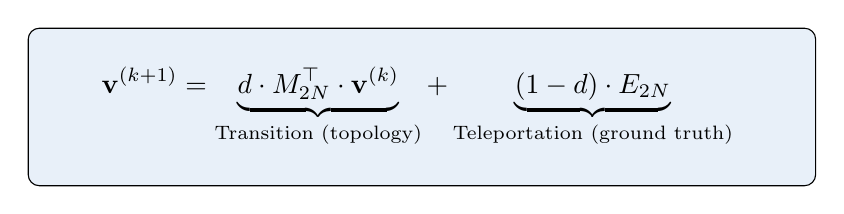
\begin{tikzpicture}
    \node[draw, rounded corners, fill=accent!10, minimum width=10cm,
          minimum height=2cm, align=center] {
      $\displaystyle\mathbf{v}^{(k+1)}
      = \underbrace{d \cdot M_{2N}^\top \cdot \mathbf{v}^{(k)}}_{\text{Transition (topology)}}
      + \underbrace{(1-d) \cdot E_{2N}}_{\text{Teleportation (ground truth)}}$
    };
  \end{tikzpicture}

  \medskip
  \small
  \begin{tabular}{lll}
    \toprule
    \textbf{Component} & \textbf{Built from} & \textbf{Role}\\
    \midrule
    Transition $M_{2N}$ & Road topology, lengths, speeds
      & Where vehicles \textbf{move}\\
    Teleportation $E_{2N}$ & Ground-truth GPS counts
      & Where vehicles are \textbf{born}\\
    \bottomrule
  \end{tabular}
\end{frame}

%=================================================================
\section{Building the Transition Matrix $M_{2N}$}
%=================================================================

%─────────────────────────────────────────
\begin{frame}{The Two Phases of Driving}
  Every road link $i$ has \highlight{two states}:

  \medskip
  \begin{columns}[c]
    \begin{column}{0.44\textwidth}
      \centering
      \textbf{Up Phase}\\[4pt]
      \highlight{Actively traversing} link $i$\\[3pt]
      Stays proportional to travel time\\[3pt]
      \good{Self-loop traps mass}
    \end{column}
    \begin{column}{0.10\textwidth}
      \centering
      {\Large$\xrightarrow{\;\beta\;}$}
    \end{column}
    \begin{column}{0.44\textwidth}
      \centering
      \textbf{Down Phase}\\[4pt]
      \highlight{Locally dispersing}\\[3pt]
      Moves to adjacent links\\[3pt]
      Turning, parking, etc.
    \end{column}
  \end{columns}

  \medskip
  \centering
  $\beta = 0.90$: drop probability from Up to Down per step
\end{frame}

%─────────────────────────────────────────
\begin{frame}{Up Phase: Travel-Time Self-Loops}
  \begin{columns}[T]
    \begin{column}{0.52\textwidth}
      A vehicle on link $i$ has traversal time
      $t_i = \ell_i / s_i$ seconds.

      \medskip
      We add a \highlight{self-loop} so the vehicle ``dwells''
      on the link proportionally:
      \[
        \boxed{w_i = \mu \cdot \frac{\ell_i}{s_i}}
      \]
      \vspace{-6pt}
      \begin{itemize}\itemsep2pt
        \item $\ell_i$ = road length, $s_i$ = speed limit
        \item $\mu = 20$ = dwell-time scale
      \end{itemize}

      \medskip
      \good{Longer/slower roads retain more mass}
    \end{column}
    \begin{column}{0.45\textwidth}
      
\includegraphics[width=\textwidth]{fig1_selfloop_prob.png}
    \end{column}
  \end{columns}
\end{frame}

%─────────────────────────────────────────
\begin{frame}{Self-Loop Probability}
  \small Row-stochastic transition after adding self-loop:
  \vspace{-2pt}
  \[
    P_{\text{self}}(i, i) = \frac{w_i}{w_i + \deg^+(i)},
    \quad
    P_{\text{self}}(i, j) = \frac{A_{ij}}{w_i + \deg^+(i)}
  \]
  \vspace{-8pt}
  \centering
  
\includegraphics[width=0.55\textwidth]{fig2_mass_retention.png}
\end{frame}

%─────────────────────────────────────────
\begin{frame}{The $2N \times 2N$ Block Matrix}
  \begin{columns}[T]
    \begin{column}{0.48\textwidth}
      \[
        \boxed{M_{2N} = \begin{pmatrix}
          (1{-}\beta)\,P_{\text{self}} & \beta\,I\\
          0 & P_{\text{adj}}
        \end{pmatrix}}
      \]

      \medskip
      \begin{itemize}\itemsep4pt
        \item \highlight{Top-left}: Up$\to$Up\\
              (stay driving, with self-loops)
        \item \highlight{Top-right}: Up$\to$Down\\
              (drop to local dispersal)
        \item \highlight{Bottom-right}: Down$\to$Down\\
              (move to adjacent links)
        \item Bottom-left: $0$\\
              (no return from Down to Up)
      \end{itemize}
    \end{column}
    \begin{column}{0.49\textwidth}
      
\includegraphics[width=\textwidth]{fig5_block_matrix.png}
    \end{column}
  \end{columns}
\end{frame}

%─────────────────────────────────────────
\begin{frame}{Key Fact: $M_{2N}$ Uses \underline{No} Ground Truth}
  \centering
  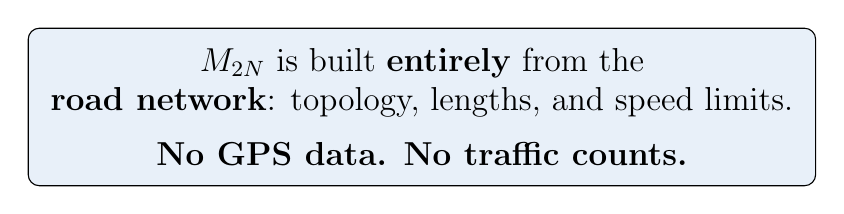
\begin{tikzpicture}
    \node[draw, rounded corners, fill=accent!10, minimum width=10cm,
          minimum height=2cm, align=center, font=\large] {
      $M_{2N}$ is built \textbf{entirely} from the\\
      \textbf{road network}: topology, lengths, and speed limits.\\[6pt]
      \textbf{No GPS data. No traffic counts.}
    };
  \end{tikzpicture}

  \bigskip
  The transition matrix defines the ``physics''---\\
  the rules of how vehicles move through the network.\\[6pt]
  It is \highlight{built once} for a city and \highlight{reused}
  for every 15-minute prediction window.
\end{frame}

%=================================================================
\section{Building the Teleportation Vector $E_N$}
%=================================================================

%─────────────────────────────────────────
\begin{frame}{Four-Step Construction of $E_N$}
  \begin{enumerate}
    \item \textbf{Extract raw GPS counts} $\mathbf{c} \in \mathbb{Z}_{\geq 0}^N$
          \hfill {\small (most $c_i = 0$)}
    \item \textbf{Laplace pseudo-count:}
          $\tilde{c}_i = c_i + 0.1$
          \hfill {\small (eliminate zeros)}
    \item \textbf{Graph-diffusion smoothing ($\gamma = 0.26$):}
      \[
        c_{\text{smooth}} = 0.74\,\tilde{\mathbf{c}}
        + 0.26\,P_{\text{adj}}\,\tilde{\mathbf{c}}
      \]
    \item \textbf{$L^1$-normalise:}
      \[
        E_N[i] = \frac{c_{\text{smooth},i}}{\sum_j c_{\text{smooth},j}},
        \qquad \sum_i E_N[i] = 1
      \]
  \end{enumerate}

  \medskip
  \begin{block}{Result}
    $E_N[i]$ = probability that a new vehicle appears on link $i$
  \end{block}
\end{frame}

%─────────────────────────────────────────
\begin{frame}{Worked Example: 5-Link Network}
  \centering
  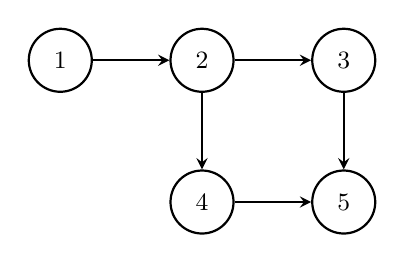
\begin{tikzpicture}[
    node distance=1.8cm, >=stealth, thick,
    every node/.style={circle, draw, minimum size=8mm, font=\small}
  ]
    \node (1) {1};
    \node (2) [right of=1] {2};
    \node (3) [right of=2] {3};
    \node (4) [below of=2] {4};
    \node (5) [right of=4] {5};
    \draw[->] (1) -- (2);
    \draw[->] (2) -- (3);
    \draw[->] (2) -- (4);
    \draw[->] (3) -- (5);
    \draw[->] (4) -- (5);
  \end{tikzpicture}

  \medskip
  \small
  \begin{tabular}{lccccc}
    \toprule
    & Link 1 & Link 2 & Link 3 & Link 4 & Link 5\\
    \midrule
    Raw count $c_i$ & 0 & 5 & 0 & 3 & 0\\
    + Laplace $\tilde{c}_i$ & 0.10 & 5.10 & 0.10 & 3.10 & 0.10\\
    Neighbour avg & 5.10 & 1.60 & 0.10 & 0.10 & ---\\
    Smoothed & 1.40 & 4.19 & 0.10 & 2.32 & 0.10\\
    \highlight{$E_N[i]$} & \highlight{0.172} & \highlight{0.516}
      & \highlight{0.012} & \highlight{0.286} & \highlight{0.012}\\
    \bottomrule
  \end{tabular}

  \medskip
  Link~1 gets \good{17.2\%} despite zero observations
  $\Rightarrow$ topology propagates evidence from its busy neighbour
\end{frame}

%─────────────────────────────────────────
\begin{frame}{Extending to $2N$: The $E_{2N}$ Vector}
  Teleportation injects vehicles only into the \highlight{Up (active)} phase:
  \[
    \boxed{E_{2N} = \begin{pmatrix} E_N \\ \mathbf{0}_N \end{pmatrix}}
    \in \mathbb{R}^{2N}, \qquad \|E_{2N}\|_1 = 1
  \]

  \bigskip
  \textbf{Physical meaning:}
  \begin{itemize}
    \item New vehicles are ``born'' actively driving on a road
    \item They naturally transition to the Down phase over time
    \item The ground truth determines \emph{where} they appear;\\
          the transition matrix determines \emph{how} they move
  \end{itemize}
\end{frame}

%=================================================================
\section{The Power Iteration}
%=================================================================

%─────────────────────────────────────────
\begin{frame}{Combining Topology + Ground Truth}
  \begin{block}{\large The Power Iteration}
    \[
      \boxed{\mathbf{v}^{(k+1)}
      = \underbrace{d \cdot M_{2N}^\top \cdot \mathbf{v}^{(k)}}_{\text{topology-driven flow (80\%)}}
      + \underbrace{(1-d) \cdot E_{2N}}_{\text{ground-truth injection (20\%)}}}
    \]
  \end{block}

  \medskip
  \begin{columns}[T]
    \begin{column}{0.48\textwidth}
      \centering\highlight{$d = 0.80$}\\[4pt]
      80\% of mass follows the\\
      \textbf{transition matrix}\\
      (roads, travel times, phases)
    \end{column}
    \begin{column}{0.48\textwidth}
      \centering\highlight{$1 - d = 0.20$}\\[4pt]
      20\% of mass is re-injected\\
      from \textbf{ground-truth GPS}\\
      (observed traffic pattern)
    \end{column}
  \end{columns}

  \medskip
  \centering
  Converges when $\|\mathbf{v}^{(k+1)} - \mathbf{v}^{(k)}\|_1 < 10^{-6}$
\end{frame}

%─────────────────────────────────────────
\begin{frame}{Convergence}
  \centering
  
\includegraphics[width=0.68\textwidth]{fig10_convergence.png}

  \small Typically converges in $\sim$40--60 iterations
\end{frame}

%=================================================================
\section{Smoothing Justification}
%=================================================================

%─────────────────────────────────────────
\begin{frame}{Why Smooth? --- The Sparsity Problem}
  \begin{columns}[T]
    \begin{column}{0.45\textwidth}
      \begin{itemize}
        \item Most links have $c_i = 0$
        \item Creates:
          \begin{itemize}
            \item MRE singularities
            \item Markov chain dead zones
            \item Biased teleportation
          \end{itemize}
        \item Without smoothing:\\
          \bad{MRE = 7{,}275}
        \item With smoothing:\\
          \good{MRE = 0.19}
      \end{itemize}
    \end{column}
    \begin{column}{0.52\textwidth}
      
\includegraphics[width=\textwidth]{fig11_sparsity_histogram.png}
    \end{column}
  \end{columns}
\end{frame}

%─────────────────────────────────────────
\begin{frame}{Graph-Diffusion as a Low-Pass Filter}
  \[
    \mathbf{c}_{\text{smooth}}
    = \underbrace{(1-\gamma)}_{\text{keep own}}
      \cdot \tilde{\mathbf{c}}
    + \underbrace{\gamma}_{\text{borrow from neighbours}}
      \cdot P_{\text{adj}}\,\tilde{\mathbf{c}}
  \]

  \medskip
  \begin{columns}[T]
    \begin{column}{0.48\textwidth}
      \centering
      \textbf{Spectral view:}\\[6pt]
      Eigenvalue of the filter:
      \[
        h(\lambda) = (1-\gamma) + \gamma\lambda
      \]
      $h(1) = 1$ \good{(preserves mean)}\\
      $h(-1) = 1-2\gamma$ \good{(attenuates noise)}
    \end{column}
    \begin{column}{0.48\textwidth}
      \centering
      \textbf{Mass conservation:}\\[6pt]
      \[
        \sum_i c_{\text{smooth},i} = \sum_i \tilde{c}_i
      \]
      Smoothing \textbf{redistributes}\\
      mass but never creates\\
      or destroys it
    \end{column}
  \end{columns}
\end{frame}

%─────────────────────────────────────────
\begin{frame}{The Bias-Variance Tradeoff}
  \begin{columns}[T]
    \begin{column}{0.42\textwidth}
      \[
        \text{MSE} = \underbrace{\text{Bias}^2}_{\uparrow\;\text{with}\;\gamma}
        + \underbrace{\text{Variance}}_{\downarrow\;\text{with}\;\gamma}
      \]
      \begin{itemize}
        \item Too little smoothing $\to$ \bad{noisy}
        \item Too much smoothing $\to$ \bad{blurred}
        \item U-shaped MSE curve
        \item Minimum \textbf{inside} the range
      \end{itemize}
    \end{column}
    \begin{column}{0.55\textwidth}
      
\includegraphics[width=\textwidth]{fig14_bias_variance_decomp.png}
    \end{column}
  \end{columns}
\end{frame}

%─────────────────────────────────────────
\begin{frame}{Cross-Validation Protocol (49 Trials)}
  \begin{enumerate}
    \item Select 49 timeframe slots (fixed seed = 42)
    \item \textbf{Split} GPS data: Set~A (train) / Set~B (test)
    \item Smooth Set~A with candidate $\gamma$
    \item \textbf{Never} smooth Set~B (oracle ground truth)
    \item Measure:
      \begin{itemize}
        \item \highlight{Predictive MSE}: smoothed A vs.\ raw B
        \item \highlight{PageRank MSE}: PageRank(A) vs.\ PageRank(B)
        \item \highlight{Pearson $r$}: correlation A vs.\ B
      \end{itemize}
    \item Average over all 49 trials
  \end{enumerate}
\end{frame}

%─────────────────────────────────────────
\begin{frame}{CV Results: MSE \& Correlation}
  \centering
  
\includegraphics[width=0.70\textwidth]{fig12_cv_mse_correlation.png}

  Both metrics optimised at \highlight{$\gamma^* = 0.26$}
\end{frame}

%─────────────────────────────────────────
\begin{frame}{CV Results: Downstream PageRank MSE}
  \centering
  
\includegraphics[width=0.70\textwidth]{fig13_cv_downstream_variance.png}

  PageRank MSE minimum \textbf{also} at $\gamma \approx 0.26$
  $\Rightarrow$ input-optimal = output-optimal
\end{frame}

%─────────────────────────────────────────
\begin{frame}{Direct vs.\ Downstream MSE}
  \centering
  
\includegraphics[width=0.82\textwidth]{fig6_smoothing_tradeoff.png}
\end{frame}

%─────────────────────────────────────────
\begin{frame}{Independent Verification (Seed = 123, 80 Splits)}
  \centering
  
\includegraphics[width=0.82\textwidth]{fig16_verification.png}

  \medskip
  \small Broad plateau at $\gamma \in [0.22, 0.30]$;
  $\gamma = 0.26$ is the \good{centre of the plateau}.\\
  MSE varies $<0.04\%$ within this band.
\end{frame}

%=================================================================
\section{Results}
%=================================================================

%─────────────────────────────────────────
\begin{frame}{Impact of Smoothing: 490-Timeframe Comparison}
  \centering
  
\includegraphics[width=0.80\textwidth]{fig15_raw_vs_smoothed_mre.png}

  \medskip
  \small
  \begin{tabular}{lcc}
    \toprule
    Pipeline & Avg MRE & Improvement\\
    \midrule
    Raw ($\gamma = 0$) & \bad{7,275} & ---\\
    Smoothed ($\gamma = 0.26$) & \good{0.19} & $\times$37,800\\
    \bottomrule
  \end{tabular}
\end{frame}

%─────────────────────────────────────────
\begin{frame}{Effect of $\mu$ (Dwell-Time Scale)}
  \centering
  
\includegraphics[width=0.64\textwidth]{fig4_mre_vs_mu.png}

  \smallskip
  MRE drops monotonically as $\mu$ increases.
  Optimal: \highlight{$\mu = 20$}
\end{frame}

%─────────────────────────────────────────
\begin{frame}{MRE Heatmap: $\mu$ vs $\beta$}
  \centering
  
\includegraphics[width=0.58\textwidth]{fig3_mre_heatmap.png}

  \smallskip
  Best combination: $\mu = 20$, $\beta = 0.90$, $d = 0.80$
\end{frame}

%─────────────────────────────────────────
\begin{frame}{Damping Sensitivity}
  \centering
  
\includegraphics[width=0.68\textwidth]{fig8_damping_sensitivity.png}

  \medskip
  $d = 0.80$ balances topology-driven flow
  with ground-truth injection
\end{frame}

%─────────────────────────────────────────
\begin{frame}{Worked Example: 4-Link Toy Network}
  \centering
  
\includegraphics[width=0.95\textwidth]{fig_toy_network.png}

  \medskip
  \small
  \begin{tabular}{lcccc}
    \toprule
    & Highway & Arterial & Connector & Local\\
    \midrule
    GPS input $E_N$ & 55\% & 25\% & 5\% & 15\%\\
    $\mu=0$ output & 32.8\% & 27.4\% & 19.7\% & 20.0\%\\
    $\mu=20$ output & \good{54.9\%} & \good{25.0\%} & \good{5.1\%} & \good{15.0\%}\\
    \bottomrule
  \end{tabular}

  \smallskip
  Self-loops \good{anchor mass} to where vehicles physically spend time
\end{frame}

%=================================================================
\section{Summary}
%=================================================================

%─────────────────────────────────────────
\begin{frame}{Final Results (49 Timeframes, Seed = 42)}
  \centering
  \begin{tabular}{lcc}
    \toprule
    \textbf{Metric} & \textbf{Value}\\
    \midrule
    Top-100 MRE & \good{0.0317}\\
    Overall MRE & \good{0.0471}\\
    \bottomrule
  \end{tabular}

  \bigskip
  \begin{tabular}{clcl}
    \toprule
    Symbol & Name & Value & Role\\
    \midrule
    $\gamma$ & Smoothing & 0.26 & Evidence propagation\\
    $\mu$ & Dwell-time & 20 & Self-loop weight\\
    $\beta$ & Phase-drop & 0.90 & Active $\to$ dispersal\\
    $d$ & Damping & 0.80 & Topology vs.\ ground truth\\
    \bottomrule
  \end{tabular}
\end{frame}

%─────────────────────────────────────────
\begin{frame}{Key Takeaways}
  \begin{enumerate}
    \item \highlight{Transition matrix} $M_{2N}$ encodes road physics:\\
          topology $+$ lengths $+$ speeds $\to$ two-phase block structure with self-loops
    \bigskip
    \item \highlight{Teleportation vector} $E_{2N}$ encodes ground truth:\\
          GPS counts $\to$ Laplace $\to$ graph-diffusion smoothing $\to$ normalise
    \bigskip
    \item \highlight{Smoothing} cross-validated at $\gamma^* = 0.26$:\\
          U-shaped MSE, input-optimal = output-optimal
    \bigskip
    \item \highlight{Final model}: Top-100 MRE = \good{0.0317},
          Overall MRE = \good{0.0471}\\
          on 49 random 15-minute timeframes from September 2018
  \end{enumerate}
\end{frame}

%─────────────────────────────────────────
\begin{frame}{}
  \centering
  \vfill
  {\Huge\highlight{Thank You}}

  \vfill
  {\large Questions?}
  \vfill
\end{frame}

\end{document}
